%% This file is generated by Jinja2
% Template for bipartite weighted matching
% Author: Long Gong
\documentclass[border=2pt]{standalone}
%%%<
\usepackage{verbatim}
%%%>
\begin{comment}
:Title: Template for bipartite weighted matching
:Author: Long Gong

A template for bipartite weighted matching. 

In some ways, this TeX script works as the "model" of our application 
for visualizing a weighted bipartite matching. 


Programmed in TikZ by Long Gong. Templating language is Jinja2, 
templaing syntax is the default setting of Jinja2.
\end{comment}


\usepackage{tikz}
\usetikzlibrary{calc,positioning}

\begin{document}
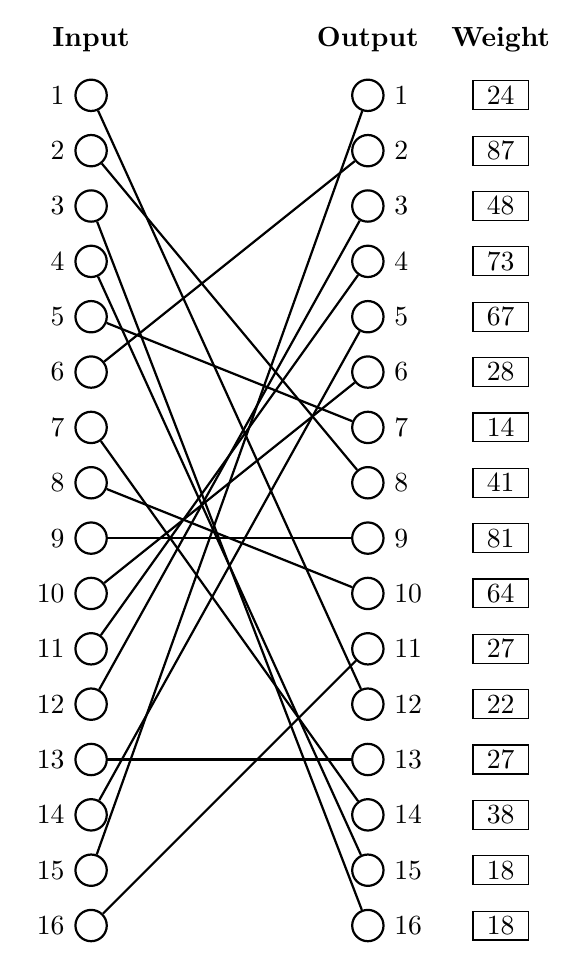
\begin{tikzpicture}[
vertex/.style={circle, draw, inner sep=4pt, thick},
edge/.style={thick},
weight/.style={rectangle, draw, inner sep=2pt, minimum width=20pt},
info/.style={draw=none,fill=none,inner sep=0pt}]

%% local variables
\def \margin{48pt}
\def \hm {100pt}
\def \vm {20pt}
\def \NUMOFVERTICES {16} 

%% place all input vertices
\foreach \s in {1,...,\NUMOFVERTICES}
      \node[vertex,label=left:$\s$] (I-\s) at (0,{- (\s - 1) * \vm}) {};

%% place all output vertices
\foreach \s in {1,...,\NUMOFVERTICES}
      \node[vertex,label=right:$\s$] (O-\s) at (\hm,{- (\s - 1) * \vm}) {};

\node[info] (I) at (0,{- (\NUMOFVERTICES - 1) * \vm}) {};
\node[info] (O) at (\hm,{- (\NUMOFVERTICES - 1) * \vm}) {};

%% place other ifnormation
\node[info] (in) at (0,\vm) {\bf Input};
\node[info] (out) at (\hm, \vm){\bf Output};
\node[info] (weight) at ({\hm+\margin}, \vm) {\bf Weight};

%% matching information
% ==========================================
% 1 12 24
% 2 8 87
% 3 16 48
% 4 15 73
% 5 7 67
% 6 2 28
% 7 14 14
% 8 10 41
% 9 9 81
% 10 6 64
% 11 4 27
% 12 3 22
% 13 13 27
% 14 5 38
% 15 1 18
% 16 11 18
% ==========================================

%% place all weight right of output vertices
\node[weight] (W-1) at ({\hm+\margin},{- (0) * \vm}) {$24$};
\node[weight] (W-2) at ({\hm+\margin},{- (1) * \vm}) {$87$};
\node[weight] (W-3) at ({\hm+\margin},{- (2) * \vm}) {$48$};
\node[weight] (W-4) at ({\hm+\margin},{- (3) * \vm}) {$73$};
\node[weight] (W-5) at ({\hm+\margin},{- (4) * \vm}) {$67$};
\node[weight] (W-6) at ({\hm+\margin},{- (5) * \vm}) {$28$};
\node[weight] (W-7) at ({\hm+\margin},{- (6) * \vm}) {$14$};
\node[weight] (W-8) at ({\hm+\margin},{- (7) * \vm}) {$41$};
\node[weight] (W-9) at ({\hm+\margin},{- (8) * \vm}) {$81$};
\node[weight] (W-10) at ({\hm+\margin},{- (9) * \vm}) {$64$};
\node[weight] (W-11) at ({\hm+\margin},{- (10) * \vm}) {$27$};
\node[weight] (W-12) at ({\hm+\margin},{- (11) * \vm}) {$22$};
\node[weight] (W-13) at ({\hm+\margin},{- (12) * \vm}) {$27$};
\node[weight] (W-14) at ({\hm+\margin},{- (13) * \vm}) {$38$};
\node[weight] (W-15) at ({\hm+\margin},{- (14) * \vm}) {$18$};
\node[weight] (W-16) at ({\hm+\margin},{- (15) * \vm}) {$18$};

%% place all edges
\foreach \i/\o in {1/12, 2/8, 3/16, 4/15, 5/7, 6/2, 7/14, 8/10, 9/9, 10/6, 11/4, 12/3, 13/13, 14/5, 15/1, 16/11}
      \draw[edge] (I-\i) -- (O-\o);

\end{tikzpicture}
\end{document}